\section{Introduction}

This first section aims to provide context to the problem explored by this thesis while also presenting the underlying objectives the presented solution intends to achieve.

\subsection{Topic Overview}

The bitcoin protocol \cite{bitcoin} defines a set of rules that enable the emergence of a decentralized peer-to-peer payment network. Nodes independently verify and subsequently store the entirety of the transaction database which is commonly reffered as the \textit{blockchain}. A system architected like bitcoin does not need to rely on trusted third parties like banks or other types of financial institutions to verify, process and distribute information, instead, this load is shared by the entire bitcoin network which uses independent cryptographic proofs as a basis for its trust model.
Embedded in the protocol is also the possibility to use bitcoin as a form of programmable money. A specific scripting language \cite{bitcoin_script} enables the user to programmaticaly dictate the conditions needed for money to be spent. Through the thoughtful manipulation of this conditions one can use the bitcoin network as a trust anchor for other systems or even as a base layer for another payment network. \\
The lightning protocol \cite{lightning_network} leverages bitcoin's programmable money concept and it defines the rules for the creation of conceptual channels with a pre-determined capacity divided between two balances that can be readjusted by the participants in the two ends of the channel, much like an abacus. A type of bitcoin payment script called \acrfull{htlc} makes multi-channel payments possible, making the network able to instantly route payments between two non neighbouring nodes. \\
The payments made between two nodes that don't share a channel are routed through the network, with the intermediate nodes, also called \textit{hops}, charging a small fee for doing helping the routing. This way in which the route path is chosen is not defined by the lightning specifications and can vary. Every implementation uses source routing, leveraging the availability of information about the topology of the network by running a version of the dijkstra algorithm with modified edge weight-metrics combined with a reputation system for channels, this can be viewed has a type of link state routing algorithm At least one implementation, ACINQ's \textit{eclair}, is also experimenting with a form of \textit{partial} source routing called \textit{trampoline routing} which will be discussed further in section \ref{sssec:trampoline_routing}. \\
After a route is successfully discovered the overlying payment can still be invalid or fail to be completed. A route might span more than 20 hops which collides with the current onion routing implementation, the channel might not have enough capacity for the payment, nodes in the payment route can be uncooperative or it might be the case that at least one of the channels in the route doesn't have the right distribution of funds. This last case will be one of the main focuses of this work.

\subsection{Motivation}

Although some details about the channels and a local view of the network's topology are maintained through the peer-to-peer exchange of the gossip messages defined by the specification, a node does not possess any information about the distribution of funds in channels in which it does not take part. The fact that the information on these channel fund distributions is held privately by the partakers of each channel preserves a degree of privacy in the network while diminishing the efficiency of the routing process and contributing to the general unbalance of the channels in the network. \\
A previous analysis of the lightning network \cite{ln_analysis} concluded that when using the current Dijkstra algorithm for route finding a small increase in the volume of a payment sharply decreases its probability of success. This happens because as a payment gets larger it's harder for it to "fit" in a valid payment route, it gets more and more likely that one of the channels that make up the path doesn't have enough capacity or the right balance distribution. The solid blue line in figure \ref{fig:shortest_path_max_flow_prob} characterizes this behaviour.

\begin{figure}[H]
\begin{center}
  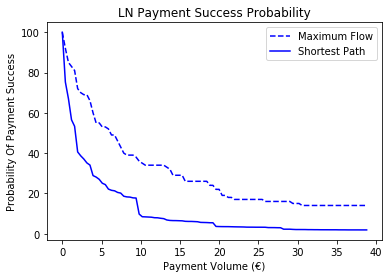
\includegraphics[width=0.6\linewidth]{images/shortest_path_max_flow_prob.png}
  \caption{Payment success probability for shortest paths and its upper bound}
  \label{fig:shortest_path_max_flow_prob}
  \end{center}
\end{figure}


The blue dotted line present in figure \ref{fig:shortest_path_max_flow_prob} takes the this concept further, characterizing the probability of success of a payment that uses a conceptual multi-path approach. Using this routing scheme a user could route a payment through all the available paths between the payer and the payee, dividing its volume between each one of them and maximizing the capacity available in the network. It's an interesting metric to look into because it can be thought as a performance upper bound and can be used to understand how much of the network's available capacity is being used by a certain routing method. To do this we find the relation between the probability of success for the shortest path routing scheme and the probability of success when using a multi-path. This relation is defined by equation \ref{eq:used_capacity}.

\begin{equation}
UC = \frac{\int_{0}^{\infty} shortestPath(V)~dV}{\int_{0}^{\infty} maximumFlow(V)~dV}
\label{eq:used_capacity}
\end{equation}

The multi-path (sometimes called multi-part) approach makes bundling the capacity of all the channels that belong to a user possible, making larger payments than any individual channel on its own would allow. In the last few months a lot of work has been done to take this concept and make it a reality and it is being currently explored through protocols like AMP \cite{amp} and implementations like c-lightning \cite{c-lightning_0.8}. Although this is a perfectly valid method for to increase the success probability of a payment in the network it won't be the focus of this work, instead this work will center itself around different single-path solutions. Given that a multi-path payments are composed of multiple single-path payments the conclusions present in the end can still prove themselves valuable when using a multi-path approach.\\
Working with an ever-growing network also poses some challenges. As the network grows keeping updated information on all the existent channel gets harder. More protocol messages need to be received, processed and relayed. Payment route finding also gets harder as the network grows. Dijkstra's algorithm, when implemented with a fibonnaci heap, has a running time complexity of $\mathcal{O}(|E| + |V|\log{}|V|)$, where $|E|$ is the number of edges and $|V|$ is the number of vertices, this means this algorithm runs in linear time with respect to $|E|$ and linearithmic time with respect to $|V|$ which indicates that as the network grows, the time taken by the route finding algorithm grows moderately with the size of the network. \\
Even though it wouldn't be expected for the current routing algorithm to have running time problems as the network scales this might still pose a challenge for smaller devices with less processing power. \\

\subsection{Objectives}
\label{ssec:objectives}

The goal of this work is to design and implement an alternative solution for efficient payment routing in the lightning network. It is essential that the solution works \gls{off-chain}, maximizes the privacy and increases payment success.
The implementation of the solution should work independently from a lightning network client, making available an API that is able to answer routing related requests.
The solution should be tested through a simulation done on a network whose topology is similar to the real network, it is expected that when si

\subsection{Thesis Outline}